\chapter{\textbf{Implementation}}

\label{chap:implementation}

In this chapter, it's discussed the virtualization design advisor implementation over OpenNebula. Our aim is to optimize the distribution of resources inside a private cloud for VM guests running database workloads. However, in order to make this work feasible, some restrictions were made. The major restriction involves the list of resources which would be modelled and optimized. In this paper, this was limited to CPU. Further restrictions were established, and they'll be explained as the advisor is detailed.

For organizational purposes and better integration with OpenNebula, our solution  is part of a module called OpenRC, which stands for Open Resource Consolidation. It was designed to work alongside OCA, since it will need full access to OpenNebula functionality. As OCA, it was also implemented in Ruby\footnote{http://www.ruby-lang.org} language. In this module, it was implemented both the steps presented in figure ~\ref{fig:architecture}, from chapter ~\ref{chap:virtualization}, and missing features from OpenNebula, needed for the advisor.

One of the missing features in OpenNebula is the ability to dynamically reallocate resources,as mentioned in chapter ~\ref{chap:infrastructure}. Although it is not supported by OpenNebula, most hypervisors currently support it for some types of resource. Besides the need for changes in the OpenNebula drivers to support these operations, it would be necessary to extend the OpenNebula's core to handle them. Instead, it was decided to implement this functionality in OpenRC, with information provided by OCA. The approach to achieve this  was the use of libvirt\footnote{http://libvirt.org/}, which defines itself as "A toolkit to interact with the virtualization capabilities of recent versions of Linux (and other OSes)". It offers an API that works with all the hypervisors supported by OpenNebula, offering many features, including CPU limitation. Currently, OpenNebula already has a libvirt API, which enables VM management over the core layer. OpenRC uses libvirt at a lower level, correspondent to OpenNebula's 
bottom layer. At this time, libvirt has three parameters that allows us to control the cpu scheduling. Here is an explanation of their use:
\begin{itemize}
 \item \textbf{quota} and \textbf{period}: These parameters work together, they allow us to set a hard limit for the cpu usage. \textbf{Period} should be in range $[1000, 1000000]$. Within it, each virtual CPU of the VM will not allowed to consume more than \textbf{quota} worth of runtime. For instance, the following values define that the VM guest will be limited to $20\%$ of CPU time:
  \begin{itemize}
   \item  \textbf{period}$=100000$; 
   \item \textbf{quota}$=20000$;
  \end{itemize}
  \item \textbf{shares}: Opposite to the previous parameters, \textbf{shares} enables us to set a soft limit for CPU usage. It specifies the proportional weighted share for the VM guest. Its value is relative. For instance, a VM configured with value $2048$ will get twice as much CPU time as a VM with value $1024$. However, if the CPU is not being used by the VM with a higher parameter value, the other will not be denied CPU idle time.
\end{itemize}

These parameters are indirectly updated and retrieved through a class called \textbf{CPULimitation}, within OpenRC. The objective of this class is to set hard/soft limits for CPU usage of OpenNebula VMs on remote hosts. Our approach to execute these remote commands  is the same as OpenNebula, in fact for this task we only import the OpenNebula's class \textbf{RemotesCommand}, which is responsible for executing OpenNebula commands through SSH\footnote{Secure Shell} on remote hosts.

Other implemented feature was the communication with the DBMS running inside the VM guest. This was achieved by the creation of the \textbf{DatabaseHelper} class. Structured according to the facade pattern, it enables access to a set of classes, responsible for establishing a database connection, set tuning parameters, process single queries or workloads, obtain estimated and actual runtime costs, etc. This pattern was chosen to make the support of other DBMSes easier in future work. For the purposes of this paper, only PostgreSQL\footnote{http://www.postgresql.org/} was supported and tested as DBMS. This decision was not only based on implementation details, but also to ease cost modelling and parameter calibration. The support of a new DBMS starts by the creation of a module, representing the DBMS. In this module,  it should be defined classes which have its functionality exposed by \textbf{DatabaseHelper}, as illustrated by figure ~\ref{fig:facade}. As these classes have database specific methods, 
they shouldn't be 
directly implemented in the facade object. For instance, when a query is run for analysing purposes, the costs are not obtained the same way for different DBMS types. Once the database module is created, following specific implementation rules, it can be easily included. 

\begin{figure}[ht]
  \centering
 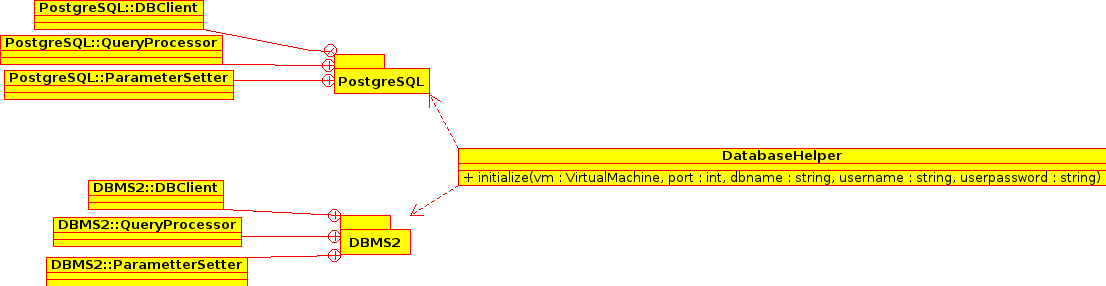
\includegraphics[scale=0.5]{database_helper_facade.png}
  \caption{DatabaseHelper facade with an eventual support of a second DBMS}
  \label{fig:facade}
\end{figure}

A \textbf{DatabaseHelper} instance needs to be initialized with a \textbf{VirtualMachine} object, defined in OCA. As mentioned in chapter ~\ref{chap:infrastructure}, OpenNebula is able to define both the MAC and IP address of a Virtual Machine, in form of a lease. It also keeps track of these leases in its SQL Pool. As any other pool element, this information can be retrieved through OCA, in XML format. So when a VM is passed to our class, it's possible to retrieve the IP address of that VM and connect to PostgreSQL. As some authentication parameters ( database name, user name, user password ) are also needed for database connection, and they are not stored by OpenNebula SQL pool, they must be passed manually to our solution.

As soon as the communication with the DBMS and the CPU limitation were implemented, it was possible to start developing modules inherent to our advisor. In the following subsections, every part of the process has its implementation detailed.

\section{Calibration}
\label{sec:calib}

The first step in order to implement the advisor is the creation of a calibration process. As discussed earlier, this task is responsible for mapping the query optimizer's cost model, which depends on its parameters $P_{i}$, to  the advisor's cost model, based on resources $R_{i}$. Without it, it's not possible to build a proper cost estimator. Since the calibration should be performed before any VM deployment on each physical host on our cloud, it was decided that this process should become an OpenNebula hook. The hook definiton is given below:
\begin{itemize}
 \item HOST\_HOOK $=$ [ \\
    name      $=$ "Calibration",\\
    on        $=$ "CREATE",\\
    command   $=$ "openrc/host\_db\_calibration.rb",\\
    arguments $=$ "\$HID",\\
    remote    $=$ no ]\\
\end{itemize}

This hook will execute the host\_db\_calibration.rb script on the OpenNebula server whenever a new host is created, passing the host id as argument. In this script, the whole calibration process is performed, as described in chapter ~\ref{chap:virtualization}. Initially, it searches for the image of a specific VM, which basically contains the calibration database. As hosts and virtual machines, images are also objects managed by OpenNebula. Thus, it needs to be added to the image pool before running the calibration script.

The calibration database running inside the VM is generated by pgbench\footnote{http://www.postgresql.org/docs/devel/static/pgbench.html}. This tool is able to run benchmark tests, based on TPC-B, for PostgreSQL. During implementation, it was only used to generate and populate our calibration database. Its choice relies on its integration with PostgreSQL, usability, and the ability to populate databases with custom sizes.

Once the calibration database is up and running, it's necessary to run specially designed queries to find out the relation between different resource allocation levels and tuning parameters costs.  As mentioned in subsection ~\ref{subsec:cost}, DBMSes don't generally share the same notion of cost. It means that we also must find the relation between DBMS estimated costs and actual costs, which would be the execution times. In PostgreSQL, all costs are normalized with the respect of time required for a single page to be fetched from disk. This cost is represented by the parameter $seq\_page\_cost$. Therefore, by finding it's actual value, we also find this relation. 


Our approach to find the actual cost values for $seq\_page\_cost$ was to use a tool to find the virtual disk throughput. In this implementation, the tool hdparm\footnote{http://sourceforge.net/projects/hdparm/} was chosen. Among other features, this utility serves as a disk benchmarking alternative for Linux. It must be previously installed in the calibration VM. Its results are obtained through a specially designed PostgreSQL function, added to the calibration database. Based on the results retrieved from this function, the cost of $seq\_page\_cost$ is calculated. Besides this calculation, it's also important to decide how to simulate I/O disk contention at this step. This would happen in production environments, where multiples VM guests are being run concurrently. Calculating $seq\_page\_cost$ without considering a realistic scenario could lead to inaccurate results. It was decided to magnify this problem by stressing the host disk while the costs are being generated and retrieved. The stress\footnote{http://freecode.com/projects/stress} utility was chosen to generate disk stress. It's used to spin several 
workers writing on files and removing directory entries on the remote host. In a more realistic setup, the VMs would compete less for I/0, and probably this cost would have a certain variability. By stressing the disk, our aim is to simulate a worst-case scenario. 


After finding the relation between the DBMS estimated cost and the actual cost ( execution time ), it's possible to calibrate the tuning parameters. Since this paper is restricted to reallocate CPU among VMs, only parameters that describe CPU need to be calibrated. For PostgreSQL, these are shown below.

\begin{table}[ht]
    \centering
    \begin{tabular}{ | l | p{5cm} |}
    \hline
    Parameter & Description  \\ \hline
    \textbf{cpu\_operator\_cost} & Cost of processing each operator or function call \\ \hline
    \textbf{cpu\_tuple\_cost} & Cost of processing one tuple (row) \\ \hline
    \textbf{cpu\_index\_tuple\_cost} & Cost of processing each index entry during an index scan  \\
    \hline
    \end{tabular}
    \caption{Parameters that describe CPU}
    \label{table:descriptive}
\end{table}


PostgreSQL uses these parameters to build its query optimizer's cost estimates. That's why a lot of documentation can be found on how to tune these parameters in order to obtain better cost execution plans. However, the way these parameters are exactly used within these plans is poorly documented. Only by observing the source code is possible to determine how they are applied to simple query plans. The first two parameters at table ~\ref{table:descriptive}, $cpu\_tuple\_cost$ and $cpu\_operator\_cost$ can be obtained by the query presented at subsection ~\ref{app:cal1}. Without changing the values of any PostgreSQL's default parameter values, this query will always have the same execution plan generated. It will access the table $pgbench\_accounts$ using a sequential scan, and subsequently perform an aggregation. PostgreSQL has the following equations for these two operations:
\begin{equation}
  \begin{split}
      SEQSCAN &= ( seq\_page\_cost * num\; pages \; fetched ) + ( cpu\_tuple\_cost * number\; rows ) \\
      AGGREGATE &= SEQSCAN + ( cpu\_operator\_cost * number\; rows) \\
  \end{split}
\end{equation}

The estimated cost and execution times for these equations can be obtained by executing this query on PostgreSQL with the command $EXPLAIN (ANALYZE)$. In this case, the query will be actually executed and an execution plan will be returned. Each step in the execution plan has its corresponding costs indicated. This means that it's possible to isolate costs for each operation from the total. Based on the actual costs returned, our script is able to deduct the parameters from the equations. However, by retrieving these costs we get a different scale, as the actual costs are in milliseconds, instead of page fetches. We use the actual value of $seq\_page\_cost$ to make conversions between different scales. The equation is given below:
\[
 param_{estimated} = \frac{param_{actual}}{seq\_page\_cost_{actual}}
\]

To calculate the first two descriptive parameters, only one modification to the original equation was made. PostgreSQL considers the cost fetching pages  during a $SEQSCAN$. The problem is to determine how many pages were actually fetched from disk. One approach would be running the query with the command $EXPLAIN (ANALYZE,BUFFERS)$. By using this command, it's informed the number of pages hit in the PostgreSQL cache and number of pages that needed to be read. However, the PostgreSQL cache may not reflect the state of the operating system cache. During experimentations, changes in the hit/miss ratio did not incur in an expected change in actual costs. Our approach was to cache all the data for the consults and limit the number of page accesses of a determined query. After doing that, costs related to disk page fetches were ignored from the equation.

The third descriptive parameter, $cpu\_index\_tuple\_cost$ , is used during index scans. It can be obtained through the query presented in subsection ~\ref{app:cal1}. Before running this query, it is necessary to set the following parameter:
\[
 enable\_seqscan=off
\].
This will force the planner to use an index scan plan, as $aid$ is a primary key, instead of a sequential scan. Its equation is much more complex than the previous one. Mainly because it involves a lot of I/O cost estimates. In addition to $seq\_page\_cost$, its plan is highly dependable on another parameter, namely $random\_page\_cost$. It represents the cost of fetching a non-sequentially disk page. During estimation, PostgreSQL uses an approximation of pages actually fetched after accounting for cache effects. This approximation is proposed in \cite{Mackert:1989:ISU:68012.68016}. The number of fetched pages is

\begin{eqnarray*}
  PF=&& \\
  &min(2TNs/(2T+Ns),T)\qquad \qquad \qquad & when\quad T \le b \\
  &2TNs/(2T+Ns) & when \quad (T > b) \wedge (Ns \le 2Tb/(2T-b)) \\
  &b + (Ns -2Tb/(2T-b))*(T-b)/T & when \quad (T > b) \wedge (Ns > 2Tb/(2T-b)) \\
\end{eqnarray*}
where
\begin{description}
 \item T $=$ number of pages in table;
 \item N $=$ number of tuples in table;
 \item s $=$ selectivity $=$ fraction of table to be scanned;
 \item b $=$ number of buffer pages available.
\end{description}

For the same reasons why I/O cost was discarded for the first equation, we decided to eliminate it from the $cpu\_index\_tuple\_cost$ calculation. Since we are only interested in CPU cost, instead of I/0, we cache all the data to be retrieved and consider the following parameters to be
\begin{equation}
 \begin{split}
  seq\_page\_cost &= 0 \\
  random\_page\_cost &= 0
 \end{split}
\end{equation}

Given this configuration, the equation for a single index scan can be defined as
\begin{eqnarray*}
  \lefteqn{Cost=} \\
  &&ntuples * ( cpu\_index\_tuple\_cost + qual\_op ) + \\
  &&100*cpu\_operator\_cost + \\
  &&cpu\_per\_tuple\_cost * ntuples + ( I/0\;Cost ) \\
  \lefteqn{qual\_op=} \\
  &&cpu\_operator\_cost * ncond \\
  \lefteqn{cpu\_per\_tuple\_cost=} \\
  &&cpu\_tuple\_cost + cpu\_operator\_cost * nfilters
\end{eqnarray*}
,where
\begin{description}
 \item ntuples $=$ number of tuples retrieved;
 \item ncond $=$ number of index conditions;
 \item nfilters $=$ number of filters ( including index conditions );
 \item I/O cost $=$ indicates the cost of fetching pages from disk, related to parameters $seq\_page\_cost$ and $random\_page\_cost$. As it is discarded by the calibration process, it won't be detailed.
\end{description}

The values for $cpu\_tuple\_cost$ and $cpu\_operator\_cost$, the details about our calibration query and database are already known. As we discared the I/O cost from our equation, there is only one variable left to be deducted, that is $cpu\_index\_tuple\_cost$. The calibration process then isolates this variable from the rest of the equation and finds its value under different resource allocations, like it was done for the two first parameters. The library built to enable CPU limitation is used here to set a hard limit for CPU usage.

The execution costs found during the calibration step are then stored in files, with the corresponding CPU allocation levels. The collected data is used later by the virtualization design advisor. 

\section{Virtualization Design Advisor}

After the end of the calibration process for a certain host, the virtualization design advisor can start handling database workloads and resource allocation levels. The advisor modules, shown in figure ~\ref{fig:architecture}, served as a base on how to organize our implementation. This can be seen on figure ~\ref{fig:advisor}. Here, a new process was added, namely \textbf{LoadGenerator}.  Its task is to run the workloads under resource allocations conditions established during \textbf{GreedySearch}. The costs obtained through execution are passed to both \textbf{OnlineRefinement} and \textbf{DynamicConfigurationManagement}. During workload execution, this class may call \textbf{GreedySearch} several times for reallocation, regarding changes in the workload or recurrent allocation optimizations. In this section, each class within the advisor will be detailed.


\begin{figure}[ht]
\centering
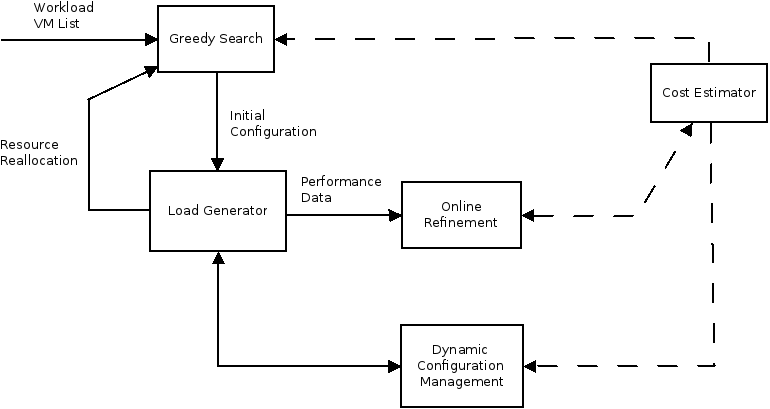
\includegraphics[width=0.8\textwidth]{advisor-arch.png}
\caption{Implementation overview}
\label{fig:advisor}
\end{figure} 

\subsection{Greedy Search}

The \textbf{GreedySearch} class, from which the advisor is started,  is an implementation of the algorithm presented in section ~\ref{sec:greedy}. This is the only class that actually changes the resource allocation levels. Considering that a private cloud is composed of multiple hosts, it is necessary to run multiple instances of this class. It was created a daemon to manage these multiple searches. It waits for virtual machines to be started and also for workloads to be run on these VMs. Then it resends this information to the \textbf{GreedySearch} instance that corresponds to the host in which that particular VM was designated to be run. Information about newly created VMs can be automatically added as soon as they are created, through a OpenNebula hook. On the other hand, workloads are sent with a script, which sends their information through a TCP Socket, in an expected format.

The search is used in three occasions. The first is when the advisor is started. The objective, in this case, is to find a better initial allocation than the default ( i.e. find an allocation of resources for the $N$ VM guests better than the proportion $\frac{1}{N}$ ). It relies on estimates provided by the \textbf{CostEstimator} class to accomplish it. In a production environment, a good approach would be to base these estimates in a workload history. As we only have a testing scenario, it was opted to base our search on the first workload that is yet to be run.

In the other two occasions, the search is called by the \textbf{LoadGenerator} class. The first is related to the online refinement process, described in subsection ~\ref{subsec:ref}. As the cost estimator model is refined after each workload execution, new calls are made to reflect these refinement changes in the resource allocation. In this case, the searches are not restarted from the default allocation, instead we search for improvements to the current allocation. If the allocation remains the same, this search will not be called any longer by \textbf{LoadGenerator}. And finally, the last occasion happens when a workload change is detected. Then \textbf{LoadGenerator} calls this class, and the search will be started from scratch. This case is similar to the first search, as both of them start from the default allocation and the cost model is restarted.

Independently on how the search is called, it always ends by applying the resource allocation levels found. \textbf{GreedySearch} is the only class within the advisor that actually changes them. This is applied in two steps. The first corresponds to setting a soft limit on the CPU level for each VM, according to the resource allocation levels found during search. The second step is to set the parameters for each DBMS, also according to the search. After they are applied, the rest of the workload can be run.

\subsection{Cost Estimator}

The cost estimation process is performed by the class \textbf{CostEstimator}. The description of how this task should be performed in the virtualization design advisor is given in subsection ~\ref{subsec:cost}. Basically, it needs to provide an estimated cost for running a certain workload under a determined resource allocation level. During initial calls to this estimator, the cost model is not built yet. So \textbf{CostEstimator} leaves this task to be performed by the cost estimator built inside the DBMS query optimizer. Here we face a problem described previously, while our cost model depends on a resource allocation $R_{i}$, the query optimizer cost estimates depend on a set of tuning parameters $P_{i}$. This mapping has already been performed in the calibration process. Therefore, this class collects all calibration data for the tuning parameters and uses linear regression on the observed points. 

The equations obtained through linear regression for each parameter will be used to map $R_{i}$ to $P_{i}$. Besides being useful to the \textbf{CostEstimator} class, they also help the \textbf{GreedySearch} class to know how to set the DMBS parameters under a certain resource allocation level. They stop being used for cost estimation purposes when the cost model is built. Our approach to build the cost model is by keeping statistics of previous calls to this class. During an initial search, \textbf{CostEstimator} may be called several times for different resource allocation levels, and so the estimated results are stored. Before running the workload, a linear regression is performed on these points. As in \cite{Soror:2008:AVM:1376616.1376711} CPU is described as a resource that varies linearly, a linear regression model provides a good approximation. After building the cost model, this class stops calling PostgreSQL for estimates. This significantly reduces the extra calls to the DBMS. So the advisor is expected to have a better performance as it is being run.

Other difference between our cost estimator and the one built inside the query optimizer is the scale used. Our approach was to use use costs based on query runtime. The reason is that this is easy to determine and a better approach to compare different DBMSes. As already mentioned in section ~\ref{sec:calib}, PostgreSQL has a different notion of cost. Like it was done during the calibration process, we simply use the actual value of $seq\_page\_cost$ to convert between the two scales. Our renormalization equation is
\[
 Cost(W_{i}, [r_{i}]) = Cost_{DB}(W_{i},P_{i},D_{i}) * seq\_page\_cost_{actual}
\]

. Once the cost model is built and the we are able to renormalize the cost, it can be refined by the \textbf{OnlineRefinement} class.

\subsection{Online Refinement}

The online refinement process adopted in our advisor is straightforward. Considering that the CPU has a linear model and that we only need to refine this resource, the \textbf{OnlineRefinement} class  is an implementation of the first refinement equation presented in subsection ~\ref{subsec:ref}. This equation is designed specifically for refining resources with linear variation. During execution, the cost model is refined the following way:
\begin{equation}
 \begin{split}
   Cost(W_{i}, [r_{i}]) & = \frac{\alpha_{i}}{r_{i}} +\beta_{i} \\
   Cost'(W_{i}, [r_{i}]) & = \frac{Act_{i}}{Est_{i}} * \frac{\alpha_{i}}{r_{i}} + \frac{Act_{i}}{Est_{i}} * \beta_{i} = \frac{\alpha_{i}'}{r_{i}} +\beta_{i}' \\
   Cost''(W_{i}, [r_{i}]) & = \frac{Act_{i}}{Est_{i}} * \frac{\alpha_{i}'}{r_{i}} + \frac{Act_{i}}{Est_{i}} * \beta_{i}' = \frac{\alpha_{i}''}{r_{i}} +\beta_{i}'' \\
    & \vdots
 \end{split}
\end{equation}

 . $\alpha_{i}$ and $\beta_{i}$ are parameters of the linear model for workload $W_{i}$, and $Act_{i}$ and $Est_{i}$ are the actual and estimated costs for running this workload, respectively. In order to apply these equations, this class needs to receive the estimated and the actual costs for this workload. The actual runtime costs are provided by the \textbf{LoadGenerator} class, and the estimated costs come from the \textbf{CostEstimator}. The latter will have then its cost model updated through the refinement performed.

\subsection{Load Generator and Dynamic Configuration Management}

The \textbf{LoadGenerator} class was added to the advisor with the objective to simply run the workloads. Besides increasing the cohesion among the advisor classes, it helps us to determine which parts of the advisor we want to enable. Both the online refinement process and the workload change detection may be disabled in order to test a specific scenario in the advisor.

This class launches a thread for each VM running on a certain host, in order to run the workloads concurrently. Each VM is designated a workload queue. Even though workload units may be received from multiple clients, they are stored in a single queue, which is processed sequentially. This definitely differentiates our tests from a production environment, where a database may receive multiple queries concurrently. It limits our advisor in testing workload intensities. Therefore, in this paper our results are focused on the workload nature, rather than its intensity. As the execution results are obtained, they are passed to \textbf{OnlineRefinement}, if it is enabled. 

While the \textbf{LoadGenerator} runs the queries for each workload, the \textbf{DynamicConfigurationManagement} monitors this execution periodically. 
It is a simplified version of the module described in subsection ~\ref{subsec:dcm}. Every monitoring period, it checks for relative changes in the cost per query. If the change is above a threshold $\theta$ ( i.e. it's a major change ), it reports it. Otherwise, the changes are ignored.

The relation between these two classes was implemented according to the observer pattern. \textbf{LoadGenerator} acts as the observer, although it only starts observing the class after all the cost models have been defined. If a major change in the workload is detected by \textbf{DynamicConfigurationManagement}, it notifies the observer . When this happens, the \textbf{LoadGenerator} class decides to restart from the greedy search process, discarding the cost model.

One of the virtualization design advisor  features that was left out in this implementation was the support of QoS parameters. This means that during execution, all the workloads are treated equally, and no retsrictions are made to their improvement or decrease in performance. The implementation of the \textit{benefitial gain factor} and the \textit{cost degradation} will be left for future work.




%In this paper, it's proposed an implementation of the virtualization design advisor over OpenNebula. The aim is to optimize the distribution of resources inside the private part of a cloud for VMs running database workloads. Since it's not possible, nor makes sense to optimize an external provider's infrastructure, the public part of the cloud is just ignored. We also stick to the PostgreSQL\footnote{http://www.postgresql.org/} as the DBMS used in our solution, although the support for other DBMSes could be extended in future work.

%As already described, the virtualization designer advisor has only been modelled and tested against one server. There are two issues in porting this solution to a cloud. First, a cloud can contain several hosts, instead of one. Other issue is that a cloud is a heterogeneous environment. In spite of the homogeneous view of resources provided by the VMM, the hosts may be different themselves. To address these problems, the proposed approach consists in having $N$ instances of our advisor, being $N$ the number of nodes in the private cloud. Therefore, the advisor will not see the cloud as a whole, but only the host it was assigned to work with, the same as it was working with only one server. 

%The first step of this implementation would be the creation of a module responsible for the calibration process. As discussed earlier, this calibration will be used to map the query optimizer's cost model, which depends on its parameters $P_{i}$, to  the advisor's cost model, based on resources $R_{i}$. This process is supposed to be executed before any VM deployment, since the initial allocation depends on the latter cost model. Thus, it will be executed whenever a new physical host is added to a cluster. As this paper is limited to one DBMS, the renormalization step will  not be performed.


%After calibration, we expect the OpenNebula's default scheduler to define which host will be assigned to the VM that is to be deployed, as usual. At this step, the only provision that needs to be taken is to set the \textit{RANK} variable properly. In this paper, we intend to deal with only two types of resources: memory and CPU. Therefore, we propose the following heuristic for the \textit{RANK}:
%\begin{itemize}
% \item \textit{RANK} $=$ $\alpha *$ \textit{FREECPU} + $ (1 -\alpha) *$ \textit{FREEMEMORY}, $  0 \le \alpha \le 1  $.
%\end{itemize}
%In this equation, we expect $\alpha$ to be used to prioritize one type of resource over another. Since the scheduler assigns the host before being possible to run the advisor, this heuristic will be used for all kinds of workloads. So it doesn't matter whether they are more or less CPU intensive or memory intensive. We consider this to be a limitation. However, we still expect that this heuristic will be able to  distribute well the VMs among the hosts.

%Once the VMs are placed on a machine, the initial configuration step from the virtualization design advisor can be started. In order to deal with their initial configuration, it's proposed the use of the greedy search algorithm, described earlier in this paper. A problem that has already been identified, which affects the greedy algorithm, is the lack of current support for dynamic resource reallocation in OpenNebula. One possible approach would be the use of libvirt\footnote{http://libvirt.org/}, which defines itself as "A toolkit to interact with the virtualization capabilities of recent versions of Linux (and other OSes)". It offers an API that works with all the hypervisors supported by OpenNebula, offering many features, including resource reallocation. Currently, OpenNebula has an libvirt API, which enables this tool to manage the VMs over the core layer. It should be possible to implement a solution by using libvirt under the core layer, to extend the drivers' capabilities too.

%The online refinement and the dynamic configuration management steps should have direct implementations, following their descriptions. The initial configuration is defined by the greedy algorithm ( the static resource allocation module ), it stops when it finds the best allocation, which may be the optimal or close to it. Once this task is performed, the online refinement is started. It updates the cost model by observing estimated and actual times of workloads.  It returns an optimized cost model to the first step, where the greedy algorithm is restarted and searches for a new recommendation with the optimized cost model. The optimizer only stops when the newly obtained recommendations don't differ from the original ones (i.e. it stabilizes ). The dynamic configuration management module is also started after the the end of the initial configuration. It also uses optimized cost models to monitor changes in the workload. It may restart the workload when major changes are detected.

%The performance of this advisor is expected to improve as optimized cost models are obtained, and so less calls to the DBMS's query optimizer are needed. This is due to the fact that these calls have a high computational cost.


